\chapter{Marco Teórico}
\epigraph{\textit{Research is what I'm doing when I don't know what I'm doing.   
	}}{\textit{— Wernher von Braun, NASA engineer}}
	\vspace*{8cm}
	\begin{center}
		\centering
		\includegraphics[width=10.5cm]{example-image}
    \end{center}
\thispagestyle{empty}
\newpage
\vspace*{2cm}
En este capítulo abordaremos algunos temas y conceptos teóricos para sentar la base necesaria del proyecto y de este modo, continuar con el diseño del proyecto.

\section{Algoritmos de predicción}
En uno de los trabajos de Galam, propone una población que evoluciona a través de un contexto con dos opciones con una probabilidad de éxito o fracaso, de un espacio de individuos cualquiera y de este espacio, dividirlos en 3 grupos generando una nueva población para evaluar a la mayoría predominante en esas particiones. \cite{Galam2008}
% Insertar diagrama del TT

En los grupos no es estrictamente necesario ser de 3 individuos, el agrupamiento de individuos puede ser de cualquier tamaño, este comportamiento puede aplicarse a distintos casos, ya que es posible evaluar el desarrollo de un comportamiento de la población.

\subsection{Modelo de reglas de la mayoría local}
Consideramos grupos, que están constituidos por la segregación aleatoria de 3 agentes. Da la probabilidad de tener un \textbf{A} elegido en el nivel \textit{(n + 1)} de un grupo de nivel \textit{n} donde $P_{n}$ es la porción de personas \textbf{A} elegidas en el n-nivel.\cite{Galam2008}
\begin{equation}
    p_{n}+1 \equiv P_{3}(p_{n}) = p_{n}^3 + 3p_{n}^2(1-p_{n})
\end{equation}
La función de votación $P_{3}(p_{n})$ tiene 3 puntos fijos $p_{d} = 0$, $p_{c,3} = 1/2$ y $p_{t} = 1$. El primero corresponde a la desaparición de A. El último punto $p_{t}$ representa la situación de la dictadura donde solo \textbf{A} esta presente. Ambos son estables. Por el contrario, $p_{c}$ es inestable. Para determinar el umbral a plena potencia. A partir de $p_{0} < 1/2$ la votación repetida conduce a (0) mientras que el flujo esta en la dirección de (1) para $p_{0} > 1/2$.\cite{Galam2008}

\begin{figure}[!ht]
    \centering
    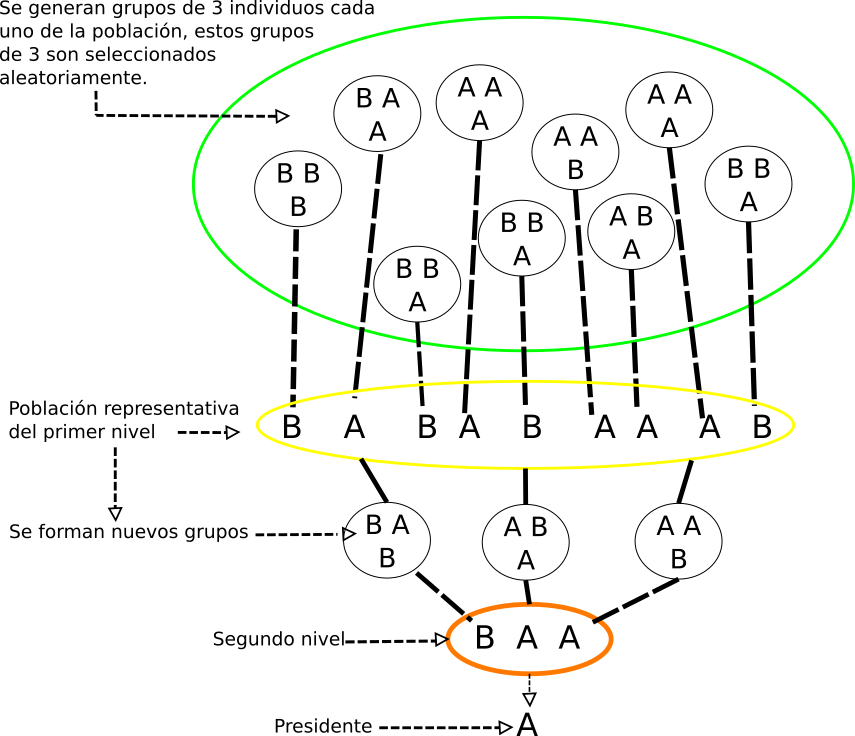
\includegraphics[scale=0.50]{TT/img/marco teorico/prediccion.png}
    \caption{Jerarquización de la población a través de diferentes iteraciones}
    \label{graphic:prediccion}
\end{figure}

Por lo tanto, la votación por regla de la mayoría produce la auto-eliminación de cualquier proporción de la tendencia \textbf{A}, mientras que $p_{0} < 1/2$, siempre que exista un número suficiente de votación, esto lo vemos en la figura \ref{graphic:prediccion}. Por consiguiente, es esencial determinar el número de niveles necesarios para garantizar el liderazgo completo a la mayor tendencia inicial. \cite{Galam2008}
%Insertar imagen describiendo el funcionamiento del algoritmo

\subsection{Grupos de votación mas grandes y la fórmula mágica}
Para grupos de votación de cualquier tamaño \textbf{\textit{r}} la función de votación $p_{n+1} = P_{r}(p_{n})$ se escribe:
\begin{equation}
    P_{r}(p_{n}) = \sum_{l=r}^{l=m} \frac{r!}{l!(r-l)!}p_{n}^{l}(1+p_{n})^{r-l},
\end{equation}
donde $m = (r + 1)/2$ para r impar y $m = (r + 1)/2$ para r par para dar cuenta del sesgo favorecido por \textbf{B}. Los dos puntos fijos estables $p_{d} = 0$ y $p_{t} = 1$ son independientes del tamaño del grupo \textbf{\textit{r}}. La inestable $p_{c,r} = 1/2$ también es independiente del tamaño del grupo \textbf{\textit{r}} para valores impares de r, para los cuales no existe sesgo. Por el contrario, varía con \textbf{\textit{r}} para valores pares. %Comienza en $p_{c,2} = 1$ para $r = 2$, disminuye a $p_{c,4} = (1 + \sqrt{13})/6 \approx 0.77$ para $\textbf{\textit{r}} = 4$ y luego sigue disminuyendo asintóticamente hacia $1/2$ desde arriba.

Cuando $p_{0} < p_{c,r}$, podemos calcular analíticamente el número crítico de niveles $n_{c}$ en los que $p_{n_{c}} = \epsilon$ siendo $\epsilon$ un número muy pequeño. Este número determina el nivel de confianza para que la predicción no tenga \textbf{A} elegido del nivel \textit{n} y superior, es decir, solo \textbf{B} sea elegido. Para hacer la evaluación, primero expandimos la función de votación $p_{n} = P_{r}(p_{n} - 1)$ alrededor del punto fijo inestable $p_{c,r}$,
\begin{equation}
    p_{n} \approx p_{c,r} + (p_{n - 1} - p_{c,r})\lambda_{r},
\end{equation}
donde $\lambda_{r} \equiv dP_{r}(p_{n})/dp_{n}|_{p_{c,r}}$ siendo $P_{r}(p_{c}) = p_{c,r}$. Esto puede reescribirse como:
\begin{equation}
    p_{n} - p_{c,r} \approx (p_{n - 1} - p_{c,r}) \lambda_{r},
\end{equation}
que luego se puede iterar para obtener
\begin{equation}
    p_{n} - p_{c,r} \approx (p_{0} - p_{c,r})\lambda_{r}^{n}
\end{equation}
El número crítico de niveles $n_{c}$ en los que $p_{n} = \epsilon$ es entonces extraído tomando el logaritmo en ambos lados para obtener,
\begin{equation}
    n_{c} \approx -\frac{ln(p_{c} - p_{0})}{ln \lambda_{r}} + n_{0},
\end{equation}
donde $n_{0} \equiv ln(p_{c,r} - \epsilon)/ln\lambda_{r}$. Poniendo en $n_{0} = 1$ mientras se toma la parte entera de la expresión produce estimaciones bastante buenas de $n_{c}$ con respecto a las estimaciones exactas obtenidas por iteraciones.

La expresión anterior es interesante pero no permite definir una estrategia ni de \textbf{A} ni de \textbf{B}, ya que la mayoría de las organizaciones tienen una estructura fija, que no se puede modificar a voluntad antes de cada nueva elección, incluso si se hace a veces. Por tanto, el número de niveles jerárquicos es fijo y constante.

Para realizar el calculo del umbral de victoria, derrota e incertidumbre de los procesos electorales se calcula a partir de una

\section{Cómputo evolutivo}
En la década de los 50's se empezó a aplicar los principios de Charles Darwin en la resolución de problemas computacionales. Diferentes corrientes de investigación independientes comenzaron a formar lo que ahora se conoce como:

\begin{itemize}
    \item Algoritmos genéticos
    \item Estrategias evolutivos
    \item Programación evolutiva
\end{itemize}

El creador de la computación evolutiva fue Lawrence J. Fogel en la década de 1960. Este desarrollo comenzó como un esfuerzo encaminado a crear inteligencia artificial basado en la evolución de máquinas de estados finitas.

Los algoritmos genéticos fueron propuestos por John H. Holland en 1975 y su motivación inicial fue la de proponer un modelo general de proceso adaptable.

Las estrategias evolutivas fueron por Ingo Rechenberg y Hans-Paul Schwefel en la década de 1970. Su principal objetivo era el de optimizar parámetros.

\section{Algoritmos genéticos}
Un algoritmo genético es una técnica de programación inspirada en la reproducción de los seres vivos y que imita a la evolución biológica como estrategia para resolver problemas de optimización. En general, los algoritmos genéticos son parte de la llamada inteligencia artificial; es decir, la resolución de problemas mediante el uso de programas de computación que imitan el funcionamiento de la inteligencia natural.\cite{Juarez2018}

Los \acrshort{AGs} fueron delineados por un par de científicos norte-americanos, Jhon Holland en los años 1970 y presentados en 1989 por David Goldberg, como un método de optimización de busqueda global, debido a que este tipo de métodos explora todo el espacio de soluciones del problema permitiendo salir de posibles óptimos locales e ir en busca de óptimos globales.\cite{Juarez2018}

\begin{wrapfigure}{r}{0.45\textwidth}
    \begin{center}
        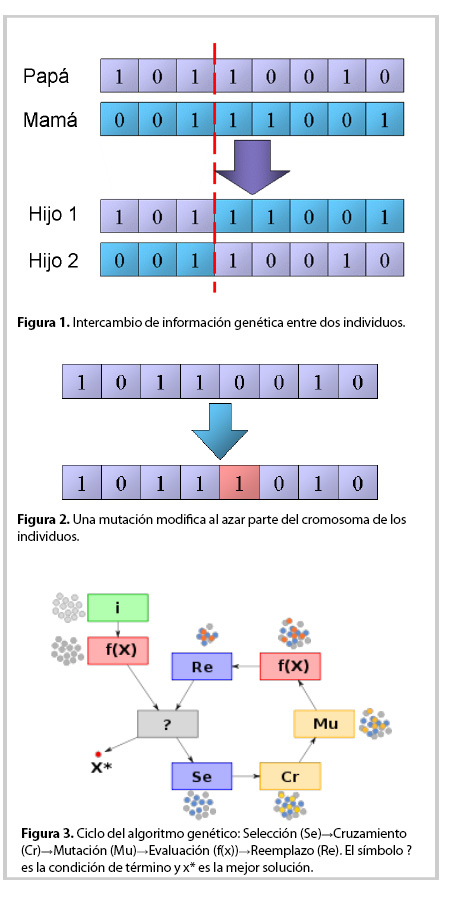
\includegraphics[width=0.45\textwidth]{TT/img/marco teorico/AGs.jpg}
        \caption{Funcionamiento de un algoritmo genético}
    \end{center}
    \label{graphic:AGs}
\end{wrapfigure}
Los \acrshort{AGs} funcionan haciendo evolucionar a individuos de una población de manera aleatoria similarmente a la evolución biológica donde las mutaciones y recombinaciones genéticas hacen que los individuos mas adaptados sobreviven y los menos aptos son descartados.

El funcionamiento \acrshort{AGs} dentro de un problema específico de optimización a resolver, requiere de un conjunto inicial de soluciones para ese problema, códificadas de alguna manera junto con una función de aptitud que permite evaluar cuantitativamente a cada solución. Ese conjunto de candidatos usualmente son generados aleatoriamente pero, también pueden ser soluciones que ya se saben que funcionan, esto con el objetivo de que el \acrshort{AGs} depure las opciones hasta escoger la mejor.

Cada una de las posibles soluciones es evaluada con una función matemática cuyo objetivo es analizar que tan viable es la solución respecto a las demás soluciones. La mayoría de las soluciones serán descartadas pero, una minoría no, ya que estas pueden mostrar parte de la solución, aunque sea débil o imperfecta y al final, estas posibles soluciones se les permite reproducirse.

Las candidatas que prometen son conservadas y se les permite reproducirse. Se hace múltiples copias de ellas y como no son perfectas, de forma aleatoria se realizan pequeños cambios o mutaciones durante el proceso de copia para garantizar que todas las soluciones sean examinadas. Posteriormente, esta descendencia forma un nuevo conjunto de soluciones posibles, para ser sometidas nuevamente a una ronda de evaluación de aptitud, seleccionando las mejores y desechando las que han empeorando. Esto se repite hasta llegar a una solución óptima. 

Resumiendo el proceso, un \acrshort{AGs} consiste en los siguientes pasos: 

\begin{itemize}
    \item \textbf{Inicialización: }Se genera de manera aleatoria una población inicial constituida por posibles soluciones al problema, también se les puede llamar individuos.
    \item \textbf{Evaluación: } Es la aplicación de la función evaluadora a cada uno de los individuos.
    \item \textbf{Evolución: } Es la fase donde se aplican los operadores genéticos (\textit{selección, reproducción y mutación}).
    \item \textbf{Final: }Sucede cuando el \acrshort{AGs} se detiene al encontrar la solución óptima al problema, aplicando criterios de evaluación, ya que generalmente esta se desconoce.
\end{itemize}
\section{Relación de algoritmos genéticos con los algoritmos de predicción}
En la siguiente sección los algoritmos genéticos serán referenciados como \acrshort{AGs} y a los algoritmos de predicción como \acrshort{APs}.

\subsection{Trabajos con poblacionales}
Ambos algoritmos trabajan con población de agentes, en el caso de \acrshort{AGs} utilizan individuos que son manejados como genes y en los \acrshort{APs} pueden ser individuos, colonias o municipios (para el caso de este trabajo terminal).

\subsection{Evolución}
Los \acrshort{AGs} utilizan la evolución a través del tiempo usando una función de evaluación, por otro lado, los \acrshort{APs} utilizarán la regla de mayoría propuesta por Serge Galam.

\section{Aleatoriedad en los algoritmos genéticos}
Los \acrshort{AGs} usan puntos de cruce con probabilidades de que muten a través de las generaciones que se vayan creando, aplicando la aleatoriedad al proceso de encontrar la solución óptima es importante en el trabajo terminal porque el comportamiento humano es aleatorio en grupos grandes.
